\documentclass[11pt]{article}
\usepackage{bookmark}
\usepackage{algorithm}
\usepackage{algpseudocode}
\usepackage{amsfonts}
\usepackage{amsmath}
\usepackage{amssymb}
\usepackage{amsthm}
\usepackage{bm}
\usepackage{color}
\usepackage{comment}
\usepackage{float}
\usepackage{graphicx}
%\usepackage[hidelinks]{hyperref}
\usepackage{makecell}
\usepackage[caption=false,font=footnotesize,subrefformat=parens,labelformat=parens]{subfig}
\usepackage{wrapfig}
\usepackage{url}
\usepackage[table]{xcolor}
\graphicspath{{images/}}
\setlength{\parindent}{0.25in}
\setlength{\parskip}{.05in}
\pagestyle{plain}
%Title, date an author of the document
\title{Progress Report}
\author{Bardia Mojra}


\begin{document}
\maketitle
\thispagestyle{empty}

\bigskip
\bigskip
\begin{center}
 Robotic Vision Lab
\end{center}

\begin{center}
The University of Texas at Arlington
\end{center}

\newpage

\section{Specific Research Goals}
\begin{itemize}
      \item VPQEKF (\textcolor{red}{May 30th}): Work on the paper.
      \item DLO Manipulation Dataset (ICRA - \textcolor{red}{Sept. 1st})
\end{itemize}

\section{To Do}
\begin{itemize}
  \item QEKF Paper - 30\% extension (\textcolor{red}{May 30th}):
  \begin{itemize}
      \item Edit VEst section and add updates.
  \end{itemize}
  \item QEKF/QuEst+VEst Implementation (\textcolor{red}{May 30th}):
  \begin{itemize}
      \item OOP Integration: QEKF - on-going.
      \item Feature point extraction: implement semantic segmentation
      \item Address scale factor (depth-scale) issues: DL solutions?
      \item Address "hand off" issue when objects enter or leave field of view
      \item Real-time streaming images for real-time operation (optional)
      \item Experiments - on-going.
      \item Noise issue: noise cannot be modeled - revisit
  \end{itemize}
  \item  DLO Manipulation:  \textcolor{red}{Sept. 1st}
  \begin{itemize}
      \item Find other ICRA dataset papers and summarize the structure. --- This week.
      \item Dataset (ICRA -  \textcolor{red}{Sept. 1st}):
      \begin{itemize}
            \item Finalize MoCap design, design digital twin work cell. --- This week.
            \item Build work cell.
            \item Collect data and create a dataset.
            \item Create object dynamics ground-truth method, format, and evaluation
            metrics.
      \end{itemize}
      \item Control and Tracking
      \begin{itemize}
            \item Create UR5+DLO simulation in Matlab and begin work on H-Infinity control before Reza leaves for Indiana State.
            \item Model dynamics and deformity
      \end{itemize}
      \item Real-Time Preception
      \begin{itemize}
        \item Implement PVnet, perform transfer learning and retrain using
        in house dataset.
        \item Time model inference, using auto-encoders generate the lowest
        dimensional representation for each object.
        \item Use another GAN model for object deformity for each object.
        \item Evaluate encoded representation for accuracy.
        \item Used another GAN to explore other abstraced representations from
        individual encoded representation. In theory, we can create a low
        dimensionsal representation for multiple similar objects, given all
        individual low-dimensional representations. This is inspired by "fundamental
        principles first" approach which has universal applicability.
      \end{itemize}
      \item
  \end{itemize}
\end{itemize}


\section{Progress}
The following items are listed in the order of priority:
\begin{itemize}
    \item VPQEKF (\textcolor{red}{RAL - April 1st, 2022}): This week, I had to
    spend couple days on the system architecture but it is complete now. Now,
    I have a complete OOP implementation in Matlab that share the same
    architecture with my Python implementation. This will allow me to easily
    reuse, integrate and run source code between the two programming languages.
    This code is also ready for field deployment since it only saves the
    estimates at run-time and performs error computation at post processing.
    The following are the results for QuEst and VEst methods compared against
    top pose and velocity estimation methods. We compared QuEst against
    Eight-Point, Nister, and Kukelova pose estimation algorithms and results are
    shown in figure [1]. Figure [2]
    shows output results for VEst module with pose estimates from mentioned
    methods. So far, we have tested our algorithm on KITII, ICL, and TUM
    benchmarks. I will add Kneip and Stewenius pose estimation methods and NAIST
    benchmark at a later time.\

    \begin{figure}
      \begin{center}
      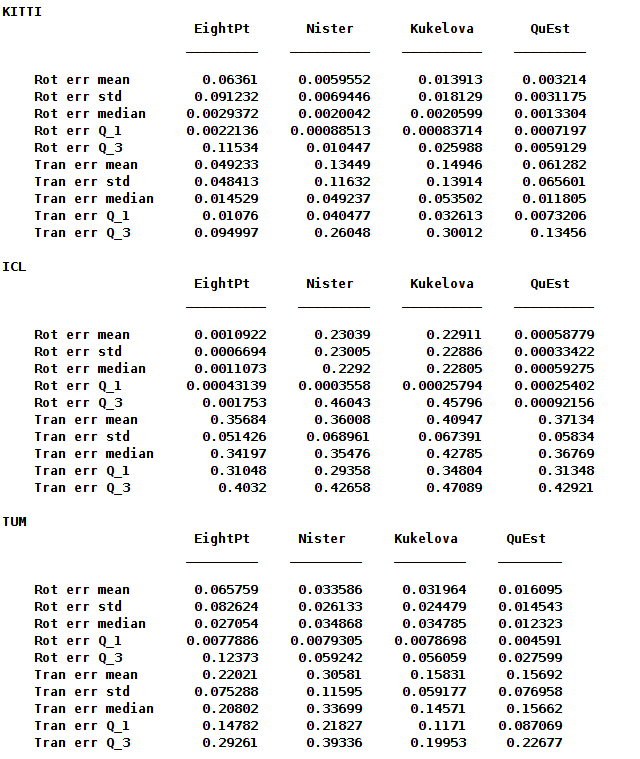
\includegraphics[width=\linewidth]{poses_n_benches.png}
      \caption{Classical Pose Estimation Methods vs. Benchmarks}
      \label{fig:poses_n_benches}
      \end{center}
    \end{figure}

    \begin{figure}
      \begin{center}
      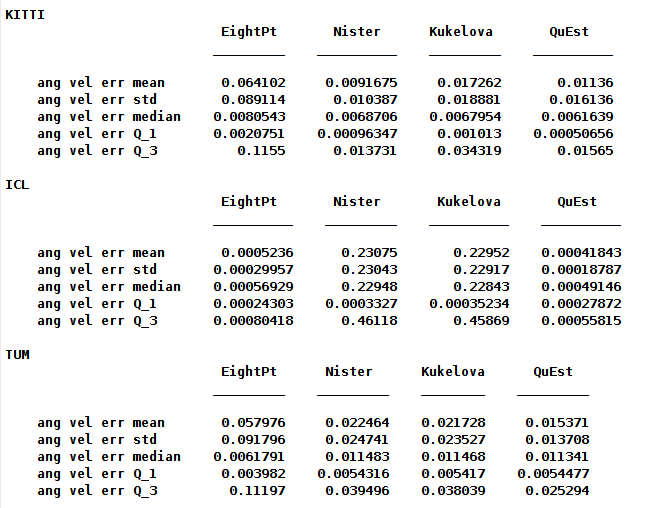
\includegraphics[width=\linewidth]{vels_n_benches.png}
      \caption{Velocity Estimation Methods vs. Benchmarks}
      \label{fig:vels_n_benches}
      \end{center}
    \end{figure}


    \item DLO Dataset: Last night, I recreated Jerry's design for the work cell
    cage, he no longer has the CAD file. I sent out a link to the file and asked
    if they want to make any changes or add anything. We will finalize the
    design this week. I reached to Sami, he seems interested and we agreed to
    meet today. I need to read more on digital twin as well as the dataset papers
    Dr. Gans and I found last week.

    \item DLO Control: No update.
    \item DLO Perception: No update.

    \item Semantic segmentation (\textcolor{blue}{DLO-02}): Per my discussion with Dr. Gans, I will explore DL methods for the depth or scale problem.
    \item Grasping Project (\textcolor{blue}{DLO-03}): I am making this a part of the DLO project.
    \item PyTorch Tutorials: Transfer learning.

  \end{itemize}

\section{Intermediate Goals - Fall 2021:}
\begin{itemize}
      \item QEKF: Finish paper.
      \item UR5e: Do the tutorials.
\end{itemize}

\newpage

%Sets the bibliography style to UNSRT and import the
\newpage
\bibliography{ref}
\bibliographystyle{ieeetr}

\end{document}
